\documentclass[aps,prd,11pt,notitlepage,nofootinbib,superscriptaddress,showkeys,letterpaper]{revtex4-1}
\usepackage{amstext,amsmath,amssymb,amsfonts,bbm, amsthm}
\usepackage[latin1]{inputenc}
\usepackage{fancyhdr}
\usepackage{graphicx}
%\usepackage{psfig,epsfig}
\usepackage{hyperref}

\usepackage{epstopdf}
\usepackage{rotating}
\usepackage{cleveref}

\usepackage{cases}
\usepackage{tabls}

\usepackage{subfigure}

\usepackage{amsthm}
\usepackage{listings}
\usepackage{url}
 
\newtheorem{theorem}{Theorem}
\newtheorem{corollary}{Corollary}

\usepackage{tikz}
\usetikzlibrary{arrows,shapes,snakes}

%\usepackage{pstricks}
\usepackage{tocvsec2}


\usepackage{color}
\newcommand{\col}{\textcolor}

%\numberwithin{equation}{section}



%% to reset paragraph counter after each new subsection
%\renewcommand{\theparagraph}{\arabic{paragraph}}
%\newcommand{\Subsection}[1]{\subsection{#1} \setcounter{paragraph}{0}}
%

\def\beq{\begin{equation}}
\def\be{\begin{equation}}
\def\ee{\end{equation}}
\def\bes{\begin{eqnarray}}
\def\ees{\end{eqnarray}}




%%%%%%%%%%%%%

\newcommand{\ds}[1]{\ensuremath{\displaystyle{#1}}}
\newcommand{\R}{\mathbb{R}}
\newcommand{\ess}[1]{\hat{#1}}
\newcommand{\fixation}{\rho}
\newcommand{\incentive}{\varphi}
\newcommand{\expectation}[1]{\left \langle {#1} \right \rangle}

%%%%%%%%%%%%%

\def\bra{\langle}
\def\ket{\rangle}
\def\f{\frac}
\def\dag{^\dagger}
\def\mone{^{-1}}
\def\tl{\widetilde}
\def\pp{\partial}
\def\nn{\nonumber}
\def\what{\widehat}

%%%%%%%%%%%%%%
%%%%%%%%%%%%%%

\def\C{{\mathbbm C}}
\def\N{{\mathbbm N}}
\def\Z{{\mathbbm Z}}
\def\R{{\mathbbm R}}

%%%%%%%%%%%%%%

\def\calA{{\mathcal A}}
\def\calC{{\mathcal C}}
\def\calF{{\mathcal F}}
\def\calG{{\mathcal G}}
\def\calH{{\mathcal H}}
\def\calL{{\mathcal L}}
\def\calM{{\mathcal M}}
\def\calN{{\mathcal N}}
\def\calO{{\mathcal O}}
\def\calT{{\mathcal T}}
\def\calV{{\mathcal V}}
\def\calZ{{\mathcal Z}}

%%%%%%%%%%%%%%

\def\arr{\rightarrow}
\renewcommand{\v}{\overrightarrow}

%%%%%%%%%%%%%%%%%%%%%%%%%%%%%%%%%%%%%%%%%%%%%%%%%%%
\begin{document}
%%%%%%%%%%%%%%%%%%%%%%%%%%%%%%%%%%%%%%%%%%%%%%%%%%%

\title{\large \bf Evolutionary Forces in the Moran Process}

\author{Marc Harper}
\affiliation{Unaffiliated}
\author{Matteo Smerlak}\email{matteo.smerlak@gmail.com}
\affiliation{Perimeter Institute for Theoretical Physics, 31 Caroline St.~N., Waterloo ON N2L 2Y5, Canada}

\date{\small\today}
%----------------------------------------------------------------------------------------
%       ABSTRACT, KEYWORDS AND ABBREVIATIONS
%----------------------------------------------------------------------------------------

\begin{abstract}
\end{abstract}
\maketitle

\section{Introduction}

Darwinian evolution is by nature a \textit{composite} dynamical process: any evolutionary change involves a combination of selection, mutation and drift. This makes causal inference in evolution much less straightforward, for every evolutionary effect has not one, but at least \textit{three} entangled causes. Delineating the respective importance of these forces in a given evolutionary change would help simplify analysis, but this seems an ill-defined problem: how much of the appearance of a new trait in a population is due to the original mutation? To its subsequent selection through differential reproduction? To drift effects? All three forces are essential components of the evolutionary process.

To make things worse, the selection component is itself of mixed nature, in the sense that it usually acts on several different levels. Examples of this are frequency and density dependence, wherein the fitness effect of a mutation depends not just on the mutant's current genotype, but also on the structure and size of the population to which it belongs. In extreme cases, individual-level and population-level notions of fitness can be opposite: a high-fitness mutant can end up \textit{decreasing} the population mean fitness, as in the prisoner's dilemma. More commonly, the task of assigning relative weights to individual-level vs. population-level selective pressures is hard to define precisely.  

The purpose of this paper is to discuss a setting where evolutionary forces actually can be decomposed quantitatively: the Moran birth-death process. The Moran process models evolving multi-type populations in terms of overlapping generations, such that each descendant population is determined stochastically from the ancestral population and pre-determined mutation rates. The population evolves until it stabilizes -- fixates in a state of all one type, if mutation is not present, or settles into a stationary state of the Markov process, moving between various population states indefinitely. \cite{}

The tool we use to define and quantify the relative strength of evolutionary forces is a general property of Markov processes which (for lack of generally accepted term) we call the \textit{yen}. This concept was originally introduced in the context of non-equilibrium statistical mechanics, where it can be interpreted as a generalization of the notion of heat. More recently, the notion of yen was showed to shed new light on various and seemingly unrelated problems, such as cell replication XXX,  wealth inequality XXX. In the context of evolutionary dynamics, yen is closely related to the notion of ``fitness flux" discussed in XXX.

An interesting feature of the yen is that is brings to light the \textit{directionality} of Markovian dynamics. In statistical mechanics, this directionality is associated to the second law of thermodynamics, and indeed the concept of yen was invented to formulate generalizations of this law. The implications of such directionality for the Moran evolutionary process will be discussed sec. \ref{direction}.

\section{The yen of a Markovian path}

Consider a Markov chain on a finite set of states $V$, characterized by transition probabilities $T:V\times V\to [0,1]$. The \textit{yen} of a path $p=(v_1,\cdots v_{\vert p \vert})\in V^n$ with length $\vert p \vert$ is defined as 

\begin{equation}
        Y(p)=\sum_{i=1}^{\vert p \vert-1}\,\ln\,\frac{T(v_i,v_{i+1})}{T(v_{i+1},v_{i})}
        %=\ln\,\frac{\prod_{i=1}^{n-1}T(v_i,v_{i+1})}{\prod_{i=1}^{n-1}T(v_{i+1},v_{i})}        
\end{equation}
with the convention $\ln(0/0)=0$. Its interpretation is simple: by comparing the forward transition probabilities $T(v_i,v_{i+1})$ with the backward transition probabilities $T(v_{i+1},v_{i})$, the yen measures the system's ``preference" for the path $p$ over its reverse $p^{-1}=(v_{\vert p \vert},\cdots,v_1)$. In this sense, the yen generalizes the notion of ``landscape" familiar from physics (energy landscape) and biology (fitness landscape) to any Markov chain: if $v$ and $w$ are two states of the chain connected by a path $p$, we can picture $v$ as ``higher" in the landscape\footnote{Here we use the biologist's convention for landscape, where peaks are attractive and valleys repulsive; physicists use the opposite convention.} than $w$ if $Y(p)<0$ and vice versa. Note that the yen is trivially odd with respect to reversal, $Y(p^{-1})=-Y(p)$. 

The yen has several remarkable properties, some of which are explored in detail in XXX. Here we would like to mention two. 

\begin{itemize}
        \item \textit{Stationary distributions}. Let $s:V\to[0,1]$ be the stationary distribution of the Markov chain, defined equivalently as the limit $\lim_{k\to\infty}T^kz$ for any initial distribution  $z:V\to[0,1]$ or as the eigenvector of the transition matrix with eigenvalue $1$, $Ts=s$. (We assume this stationary distribution exists and is unique.) Then for a path $p$,
        \begin{equation}
        Y(p)>0 \quad\textrm{iff}\quad s(v_1)<s(v_{\vert p\vert}).
        \end{equation}
        This means in particular that we can detect local maxima $v_*$
         of the stationary distribution by the condition that the yen of all length-$2$ paths starting from $v_*$ be negative. In this sense the yen can be viewed as a discrete ``derivative" of the stationary distribution. 
        
        In the special case where the Markov chain is reversible, i.e. satisfies the detailed balance condition $s(v)T(v,w)=s(w)T(w,v)$ for any pair of states $(v,w)$, we have the stronger property that 
        $Y(p)=\ln s(v_{\vert p\vert})-\ln s(v_1)$ for any path $p$. This identity may be interpreted in turn as the Markov-chain analogue of the fundamental theorem of calculus.  
        
        \item \textit{Entropy}. The entropy of a distribution $z:V\to[0,1]$ is the quantity $S(z)=-\sum_{v\in V} z(v)\ln z(v)$. Its growth in time is related to the yen by the inequality\footnote{This inequality follows from a more general identity known as the \textit{fluctuation theorem} in the physics literature.}
        \begin{equation}\label{secondlaw}
                S(T^k z)-S(z)\geq\langle-Y(p)\rangle_{k,z}
        \end{equation}
        where $T^kz$ is the evolved distribution after $k$ time steps and the bracket on the right-hand side denotes an average over all length-$k$ paths $p=(v_1,\cdots v_k)$ weighted by their probability given the initial distribution $z$, viz. $\textrm{Prob}(p)=z(v_1)T(v_1,v_2)\cdots T(v_{k-1},v_k)$. The inequality \eqref{secondlaw} is a generalization of the second law of thermodynamics to general Markov chains. It expresses the idea that Markov dynamics is statistically time-asymmetric, with the negative of the yen playing the role of ``dissipation" along any given path.
\end{itemize}


\section{Decomposing evolutionary forces in the Moran process}

Let us now see how the concept of yen and its properties can be applied to evolutionary dynamics. 


\subsection{Two population types}


\subsubsection{Two types without mutations}

We begin by considering a population with two types $A$ and $B$, with $a$ individuals of type $A$ and $b$ individuals of type $B$. We assume that the total population $a+b=N$ is fixed, so that the population state is entirely determined by the number $a$ of $A$-type individuals. We denote $\bar{a}=a/N$ and $\bar{b}=b/N=1-\bar{a}$ the corresponding fractions. Finally, we suppose that the fitness of $A$ and $B$ individuals are given by two state-dependent functions $f_A(a)$ and $f_B(a)$; the population mean fitness is $F(a)=\bar{a}f_A(a)+\bar{b}f_B(a)$. 

The two-type Moran process is then defined as a Markov chain with states $a\in\{0,\cdots N\}$ and transition probabilities
\begin{eqnarray}
        T(a,a+1)&=&(1-\bar{a})f_A(a)/F(a),\\
        T(a,a-1)&=&\bar{a}f_B(a)/F(a),\\
        T(a,a)&=&1-T(a,a+1)-T(a,a-1).
\end{eqnarray} 
This Markov chain represents the evolutionary dynamics of overlapping generations: at each time step, one individual is picked at random to die, and is replaced by a new individual with fitness-proportionate probability. It captures the effects of two of the three main forces of evolution, namely selection and drift.  

Consider now the yen of a transition $a\mapsto a+1$, i.e. $Y(a,a+1)=\ln [T(a,a+1)/T(a+1,a)]$. According to the definition of the transition probabilities above, $Y(a,a+1)$ splits into three terms:
\begin{eqnarray}
        Y(a,a+1)&=&\ln \frac{f_A(a)}{f_B(a+1)}+\ln \frac{F(a+1)}{F(a)}+\ln \frac{1-\overline{a}}{\overline{(a+1)}}.%\\
        %& \underset{N\to\infty}{\simeq} & \ln \frac{f_A(a)}{f_B(a)}+\ln \frac{F(a+1)}{F(a)}+\ln \frac{1-\overline{a}}{\overline{a}}.
\end{eqnarray}
Each term captures a different component of the evolutionary change $a\mapsto a+1$. The first term $Y_s$ depends on the relative fitness of $A$ and $B$, taking positive values when $A$ is fitter than $B$: it therefore measures the contribution of \textit{natural selection} of $A$ over $B$ in the transition $a\mapsto a+1$. The second term measures $Y_a$ the growth of the population mean fitness in the descendant population compared to the ancestral population; in this sense we can say that $Y_a$ expresses the role of \textit{collective adaptation} in favoring the transition $a\mapsto a+1$. Finally the third term $Y_d$ is independent of fitness and expresses the relative likelihood of choosing and individual of type $A$ or $B$ for death: it is the contribution of \textit{drift} to the yen of $a\mapsto a+1$. 

\subsubsection{Two types with mutations}

The two-type Moran process can be generalized to include mutations. To this effect we introduce mutation rates $\mu_{AB}(a)$ and $\mu_{BA}(a)$, giving the probabilities that a type-$A$ individual mutates into a type-$B$ individual just before being introduced into the population (and reciprocally). Typical mutation rates are $\mathcal{O}(1/N)$. %For simplicity we generally consider $\mu_{AB}(a)=\mu_{BA}(a)\equiv\mu\simeq 1/N$. 

In the presence of mutations the transition probabilities become
\begin{eqnarray}
        T(a,a+1)&=&(1-\bar{a})\, \frac{f_A(a)[1-\mu_{AB}(a)]+f_B(a)\mu_{BA}(a)}{F(a)},\\
        T(a,a-1)&=&\bar{a}\,\frac{f_B(a)[1-\mu_{BA}(a)]+f_A(a)\mu_{AB}(a)}{F(a)},\\
        T(a,a)&=&1-T(a,a+1)-T(a,a-1).
\end{eqnarray} 

Assuming that $\mu_{AB} = \mu = \mu_{BA}$, we can then decompose the yen into components for each
of the evolutionary processes, using a Taylor expansion in $\mu$:

\begin{align*} 
\sigma(\mathbf{a} \to \mathbf{a+1}) &= \underbrace{\log{\frac{\bar{f}_A(\mathbf{a+1})}{\bar{f}_{B}(\mathbf{a})}}\frac{f_A(\mathbf{a})}{f_B(\mathbf{a+1})}}_{\text{Fitness}}
 + \underbrace{\log{ \frac{(N - a - 1)(a+1)}{(N - a)(a)} } }_{\text{Drift}} \\
 &+ \underbrace{\mu \left( \frac{N-a}{a} \frac{f_B(\mathbf{a})}{f_A(\mathbf{a})} - \frac{a+1}{N-a-1} \frac{f_B(\mathbf{a+1})}{f_A(\mathbf{a+1})} \right)  }_{\text{Mutation}} 
\end{align*}


This decomposition gives us the individual contributions of each of the evolutionary
forces on the dynamics of the Markov process.
%Other decompositions are possible e.g. one may combine the adaptation and relative fitness terms into a single selection term. 


\subsubsection{Examples}

As a first example, consider the simple case where fitness is state-independent, i.e. without any density or frequency dependent effects. Also assume for simplicity that $f_A=1$ ($A$ is the ``wild type"), and denote $f_B=1+s$ the fitness of $B$ (the ``mutants"), with $s\ll 1$ a small selection coefficient. In this case the yen reduces to 
\begin{equation}
%         Y(a,a+1)\simeq s+\ln \frac{1-\overline{a}}{\overline{(a+1)}}.
        Y(a,a+1)\simeq s+\ln \frac{N-a}{a+1}.
\end{equation}
This expression is compatible with the intuitive expectation that evolution has two distinct regimes: when $a\simeq N/2$ (wild type and mutant), the drift component becomes negligible and the yen reduces to the selection coefficient ($Y\simeq s$), i.e. \textit{selection} is the dominant evolutionary force; for $a\simeq 0$ or $a\simeq N$, the selection component is negligible in the yen ($Y\simeq -\ln \overline{a}$ and $Y\simeq \ln (1-\overline{a})$ respectively), and \textit{drift} dominates evolution. In this simple setting collective adaptation of course plays no role.

Another example of a two-type Moran process is the Hawk-Dove game, in which the fitness landscape $f(a)=\big(f_A(a),f_B(a)\big)$ can be written as 
\begin{equation}
        f(a)=\begin{pmatrix}
                1 & q\\
                q & 1
        \end{pmatrix}\begin{pmatrix}
                a\\
                b
        \end{pmatrix},
\end{equation} 
where $q>1$ is a fixed parameter. 


 
% \subsection{Two population types with mutations}
% 
% The two-type Moran process can be generalized to include mutations. To this effect we introduce two (in general state-dependent) mutation rates $\mu_{AB}(a)$ and $\mu_{BA}(a)$, giving the probabilities that a type-$A$ individual mutates into a type-$B$ individual just before being introduced into the population (and reciprocally). For simplicity we generally consider $\mu_{AB}(a)=\mu_{BA}(a)\equiv\mu\simeq 1/N$. 
% 
% In the presence of mutations the transition probabilities become
% \begin{eqnarray}
%         T(a,a+1)&=&(1-\bar{a})\, \frac{f_A(a)[1-\mu_{AB}(a)]+f_B(a)\mu_{BA}(a)}{F(a)},\\
%         T(a,a-1)&=&\bar{a}\,\frac{f_B(a)[1-\mu_{BA}(a)]+f_A(a)\mu_{AB}(a)}{F(a)},\\
%         T(a,a)&=&1-T(a,a+1)-T(a,a-1).
% \end{eqnarray} 
%We can condense these expressions by defining a mutation matrix
%\begin{equation}
%       M(a)=\begin{pmatrix}
%  1-\mu_{AB}(a) & \mu_{BA}(a)\\
%  \mu_{AB}(a) & 1-\mu_{BA}(a)
%\end{pmatrix}
%\end{equation}
%and a fitness vector $f(a)=\big(f_A(a),f_B(a)\big)$, such that 
%\begin{equation}
%               \begin{pmatrix}
%  T(a,a+1) \\
%  T(a,a-1) 
%\end{pmatrix}=\textrm{diag}(1-\overline{a},\overline{a})\cdot M(a)\cdot f(a).
%\end{equation}

% \begin{align*} 
% \sigma(\mathbf{a} \to \mathbf{a+1}) = \underbrace{\log{\frac{\bar{f}_A(\mathbf{a+1})}{\bar{f}_{B}(\mathbf{a})}}}_{\text{Adaptation}}
%  &+ \underbrace{\log{\frac{f_A(\mathbf{a})}{f_B(\mathbf{a+1})}}}_{\text{Relative Fitness}}
%  + \underbrace{\log{ \frac{(N - a - 1)(a+1)}{(N - a)(a)} } }_{\text{Drift}} \\
%  &+ \underbrace{\mu \left( \frac{N-a}{a} \frac{f_B(\mathbf{a})}{f_A(\mathbf{a})} - \frac{a+1}{N-a-1} \frac{f_B(\mathbf{a+1})}{f_A(\mathbf{a+1})} \right)  }_{\text{Mutation}} 
% \end{align*}


For a concrete example, consider a fitness landscape given by a Hawk-Dove game matrix,
\[ f(\mathbf{a}) = \left(\begin{matrix}
              1 & 2\\
              2 & 1\\
             \end{matrix}\right) \mathbf{a},
\]
we can plot the relative contributes of each evolutionary process (see Figure \ref{figure_HD} 3.png). When the yen is zero the stationary distribution has a local maximum at the center state $(N / 2, N / 2)$ if $N$ is even, which is the evolutionarily stable state for the landscape. Drift is largest (in absolute value) near the boundary, as are the other components, with adaptation being the smallest typically. When the game matrix is altered to another member of the Hawk-Dove class (4.png):
\[ f(\mathbf{a}) = \left(\begin{matrix}
              1 & 3\\
              2 & 1\\
             \end{matrix}\right) \mathbf{a},
\]
the yen is again zero at the stationary maximum (approximately $a=12$), and the relative fitness becomes a more dominant influence on the left boundary. With a tournament selection matrix (0.png), mutation becomes by far the most influential factor on the right boundary. Mutation also drives the neutral landscape in from the boundary (1.png).

The classical Moran process has fitness landscape of the form:
\[ f(\mathbf{a}) = \left(\begin{matrix}
              r & r\\
              1 & 1\\
             \end{matrix}\right) \mathbf{a},
\]
where $r$ is the relative fitness of the first type. Figure \ref{figure_classical_moran} (2.png)
shows the decomposition in the case of $r=2$ and $N=20$. For mutation rate $\mu = 0$
the process would fixate into the two states $(N, 0)$ and $(0, N)$ with a probability
depending on $r$. For nonzero $\mu = 1 / N$ we obtain the stationary distribution
in Figure \ref{figure_classical_moran}. As the population evolves, states with more
individuals of type $A$ are favored, and we see from the decomposition that mutation
and relative fitness dominate the dynamic, with drift playing a smaller role as the
population approaches the boundary. For larger populations, drift typically plays a
diminished role, as expected.

\subsection{General Moran process}

We focus on the Moran process with mutation, as formulated in \cite{harper2016}; see also \cite{fudenberg2004stochastic}, \cite{claussen2005non}, and \cite{moran1962statistical}. Let a population  of size $N$ be composed of $n$ types $A_1, \ldots A_n$ with $a_i$ individuals of type $A_i$ so that $N = a_1 + \cdots + a_n$. We denote a population state by the tuple $\mathbf{a} = (a_1, \ldots, a_n)$ and the population distribution by $\bar{\mathbf{a}} = \mathbf{a} / N$. Define a matrix of mutations $M$, where $0 \leq M_{i j}(\mathbf{a}) \leq 1$ may be a function of the population state in general, but we will typically assume in examples that for some constant value $\mu$, the mutation matrix takes the form $M_{i j} = \mu / (n-1)$ for $i \neq j$ and $M_{i i} = 1 - \mu$. A typical mutation rate is $\mu \approx 1/N$.

The Moran process with mutation is a Markov chain on the population states defined by the following transition probabilities, corresponding to a birth-death process where birth is fitness-proportionate (with mutation) and death is uniformly random. To define the adjacent population states, let $\mathbf{i}_{\alpha,\beta}$ be the vector that is $1$ at index $\alpha$, $-1$ at index $\beta$, and zero otherwise, with the convention that $i_{\alpha \alpha}$ is the zero vector of length $n$. Every adjacent state of state $\mathbf{a}$ for the Moran process is of the form $\mathbf{a} + \mathbf{i}_{\alpha \beta}$ for some $1 \leq \alpha, \beta \leq n$---one more type $\alpha$ individual, one less type $\beta$ individual.

At a population state $\mathbf{a}$ we randomly choose an individual of type $A_i$ to reproduce proportionally to its fitness $f_i(\bar{\mathbf{a}})$, allowing for mutation of the new individual as given by the mutation probabilities. The distribution of fitness proportionate selection probabilities is given by $p(\bar{\mathbf{a}}) = M(\bar{\mathbf{a}}) \bar{\incentive}(\bar{\mathbf{a}})$; explicitly, the $i$-th component is
\begin{equation}
p_i(\bar{\mathbf{a}}) = \frac{\sum_{k=1}^{n}{\incentive_k(\bar{\mathbf{a}}) M_{k i} }}{\sum_{k=1}^{n}{\incentive_k(\bar{\mathbf{a}})}}
% p(i) = \frac{\incentive_A(i) (1 - \mu_{AB}(i)) + \incentive_B(i) \mu_{BA}(N-i)}{\incentive_A(i) + \incentive_B(i)}
\label{fitness-proportionate-reproduction} 
\end{equation}
where the function $\incentive(\bar{\mathbf{a}}) = \bar{\mathbf{a}}_i f_i(\bar{\mathbf{a}})$. This yields the transition probabilities
\begin{align}
T(\mathbf{a},\mathbf{a} + \mathbf{i}_{\alpha, \beta}) &= p_{\alpha}(\bar{\mathbf{a}}) \bar{\mathbf{a}}_{\beta} \qquad \text{for $\alpha \neq \beta$} \notag \\
T(\mathbf{a},\mathbf{a}) &= 1 - \sum_{\mathbf{b} \text{ adj } \mathbf{a}, \mathbf{b}\neq \mathbf{a}}{T(\mathbf{a},\mathbf{b})}
\label{moran_process}
\end{align}

\section{Three population types}

For populations of more than two types, there are more directions in which the
process can move, and so more yens to consider. Fixing the two components which are changing, e.g.
$(a, b, c) \to (a + 1, b, c - 1)$ for a population of three types $A$, $B$, and $C$
allows the yen to be decomposed as for two type populations, with the appropriate
substitutions of e.g. $f_C$ for $f_B$ and the population states. Instead of
one direction for yen (+ or -) in a two type population, in a three type
population there are three possible directions.

Consider the fitness landscape given by
\[ f(\mathbf{a}) = \left(\begin{matrix}
              0 & 1 & 1\\
              1 & 0 & 1\\
              1 & 1 & 0\\
              \end{matrix}\right) \mathbf{a},
\]
and the Moran process with $\mu = 3/(2N)$ and strength of selection $\beta = 0.1$.
For simplicity we assume that $N$ is divisible by 3. Then we have several local
maxima of the stationary distribution: one interior: $(N/3, N/3, N/3)$, three on
the boundary: $(0, N/2, N/2)$, $(N/2, 0, N/2)$, $(N/2, N/2, 0)$, and the three
corner points: $(0, 0, N)$, $(0, N, 0)$, $(N, 0, 0)$. Although the process is not
reversible and a closed-form of the stationary distribution can not be easily
found (if at all), we can simply check which states have the property that the
maximum of the incoming yens is negative. These all correspond to the local
maxima of the stationary distribution (see \ref{Figure_three_type}). Moreover, we
see from the max incoming yen plot that there is an ``inner boundary'' that
is rarely traversed, and that the corner points are relatively isolated, with
only mutation to kick the trajectory out. Finally, for $N=60$, three local minima
at $(3, 3, 54)$, $(3, 54, 3)$, $(54, 3, 3)$ are (properly) detected by the
maximum incoming yen.


\section{Population Dynamics on Graphs}

Variants of the Moran process where the individuals occupy vertices on a (directed)
graph are popular. The introduction of a graph is known to alter the fixation
probabilities, strength of selection, and other properties of the process
\cite{Nowak05} \cite{RepEquOnGraphs},
and we will now see that the graph structure alters the properties of the
stationary distribution and the relative strengths of evolutionary forces. Typically
two dynamics are studied, \emph{birth-death} where an
individual is selected globally in a fitness proportionate manner to replace
(possibly with mutation) one of its outgoing neighbors selected at random; or
\emph{death-birth}, where an individual is chosen uniformly at random to be
replaced and one of the incoming neighbors is selected to replace proportionally
to the fitness of the neighbors. A complete graph with birth-death dynamics
would correspond to the Moran process with mutation described above.

Adding the graph structure typically greatly increases the number of states of
the Markov process. For example, for an undirected cycle and a population of two
types of size $N$ there are $2^N$ states corresponding to all the possible
distributions of individuals about the cycle (two in each state). If the graph
is not fixed in space, the state space can be reduced by the symmetry group of
the cycle (the dihedral group) of order $2N$ to $2^{N-1} / N$. Regardless, the
state space is exponentially larger than that of the classical Moran process which
has $N+1$ states. Because the state space becomes large quickly, the stationary
distribution is difficult to study computationally, and before now, analytically.
The yen gives us a tool to discover the local extrema without having to compute
the stationary distribution directly.

As there are now many more ways in which the population can
achieve a given mix of types, the most being $\binom{2m}{m}$ for a population
distribution of $(m, m)$, there are potentially many more local maxima and
minima. In fact, an $(m, m)$ population distribution can be both a local maximum,
when the populations occupy two adjacent semi-circles of the cycle, and a local
minimum, when the individuals are of alternating type about the cycle. The yen
tells us that in first case a small mutation rate is a stabilizing force whereas
in the second case a small mutation rate leads to instability.

Let us define the transition probabilities between states on the cycle
in the two player case. At a given graph configuration with
population distribution $(a, b)$, we choose an individual to reproduce (with
mutation) globally. This does not change the selection ratio from the classical
case. Then we choose one of the neighbors to replace, and now it matters how
the population is distributed on the graph. The configuration may not change at
all, if the
replaced individual is of the same type as the outcome of the selection-mutation
step. For example, if the population state is $(m, m)$ where the the individuals
are distributed as two connected semi-circles, and individual selected for
reproduction inside one of the two semi-circles will only change the graph
configuration if a mutation occurs. However for the four vertices where the
subpopulations are adjacent, replication without mutation and into the other
subpopulation will change the configuration.

\begin{figure}
\centering

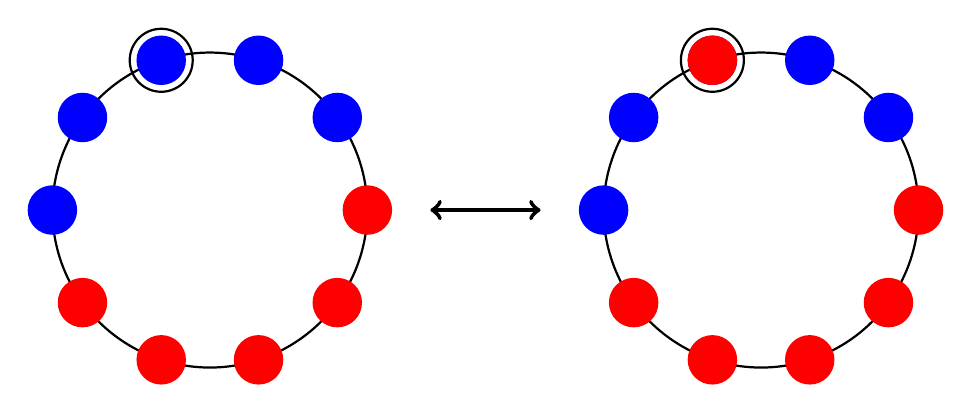
\begin{tikzpicture}[thick]

\def \n {5}
\def \radius {2cm}
\def \margin {0} % margin in angles, depends on the radius

\tikzstyle{A}=[draw=none, circle, draw=blue, fill=blue, minimum size=6mm]
\tikzstyle{B}=[draw=none, circle, draw=red, fill=red, minimum size=6mm]

\begin{scope}
% Edges
\foreach \s in {1,...,\n}
{
  \draw[-, >=latex] ({360/\n * (\s - 1)+\margin}:\radius) 
    arc ({360/\n * (\s - 1)+\margin}:{360/\n * (\s)-\margin}:\radius);
}
% Nodes
\foreach \s in {1,...,\n}
{
  \node[A] at ({180/\n * (\s)}:\radius) {};
  \node[B] at ({180/\n * (\s + \n)}:\radius) {};
}
\node[circle, draw=black, minimum size = 8mm] at ({180/\n * (3)}:\radius) {};

\end{scope}
% Arrow between the two cycles
\draw [<->, ultra thick] (2.8, 0) -- (4.2, 0);

\begin{scope}[xshift=7cm]
% Edges
\foreach \s in {1,...,\n}
{
%   \node[draw, circle] at ({360/\n * (\s - 1)}:\radius) {$\s$};
  \draw[-, >=latex] ({360/\n * (\s - 1)+\margin}:\radius) 
    arc ({360/\n * (\s - 1)+\margin}:{360/\n * (\s)-\margin}:\radius);
}
% Nodes
\foreach \s in {1,...,\n}
{
  \node[A] at ({180/\n * (\s)}:\radius) {};
  \node[B] at ({180/\n * (\s + \n)}:\radius) {};
}
% Overwrite one red with a blue
\node[B] at ({180/\n * (3)}:\radius) {};
\node[circle, draw=black, minimum size = 8mm] at ({180/\n * (3)}:\radius) {};
\end{scope}
\end{tikzpicture}
\caption{Transition showing two connected subpopulations where one population
is separated by a mutation.}
\label{transition_1}
\end{figure}

\begin{figure}
\centering
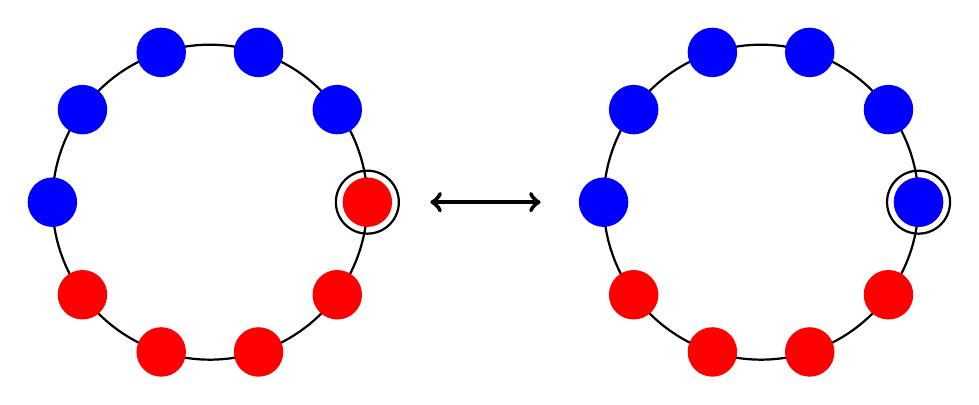
\begin{tikzpicture}[thick]

\def \n {5}
\def \radius {2cm}
\def \margin {0} % margin in angles, depends on the radius

\tikzstyle{A}=[draw=none, circle, draw=blue, fill=blue, minimum size=6mm]
\tikzstyle{B}=[draw=none, circle, draw=red, fill=red, minimum size=6mm]

\begin{scope}
% Edges
\foreach \s in {1,...,\n}
{
%   \node[draw, circle] at ({360/\n * (\s - 1)}:\radius) {$\s$};
  \draw[-, >=latex] ({360/\n * (\s - 1)+\margin}:\radius) 
    arc ({360/\n * (\s - 1)+\margin}:{360/\n * (\s)-\margin}:\radius);
}

% Nodes
\foreach \s in {1,...,\n}
{
  \node[A] at ({180/\n * (\s)}:\radius) {};
  \node[B] at ({180/\n * (\s + \n)}:\radius) {};
}

\node[circle, draw=black, minimum size = 8mm] at ({180/\n * (0)}:\radius) {};

\end{scope}
% Arrow between the two cycles
\draw [<->, ultra thick] (2.8, 0) -- (4.2, 0);

\begin{scope}[xshift=7cm]
% Edges
\foreach \s in {1,...,\n}
{
%   \node[draw, circle] at ({360/\n * (\s - 1)}:\radius) {$\s$};
  \draw[-, >=latex] ({360/\n * (\s - 1)+\margin}:\radius) 
    arc ({360/\n * (\s - 1)+\margin}:{360/\n * (\s)-\margin}:\radius);
}

% Nodes
\foreach \s in {1,...,\n}
{
  \node[A] at ({180/\n * (\s)}:\radius) {};
  \node[B] at ({180/\n * (\s + \n)}:\radius) {};
}

% Overwrite one red with a blue
\node[A] at ({180/\n * (0)}:\radius) {};
\node[circle, draw=black, minimum size = 8mm] at ({180/\n * (0)}:\radius) {};
\end{scope}

\end{tikzpicture}

\caption{Transition showing two connected subpopulations where one population
is extends into the other without a mutation.}
\label{transition_2}
\end{figure}

With the yen we can show that for the Hawk-Dove fitness landscape that this
population state is a local maximum when mutation is small, and that for the neutral
fitness landscape that there is a plateau of states connected to this one that
form a collective extrema. We need to show that the yen of each possible
transition is negative. Suppose $(a, b) = (m, m)$, $m > 4$, and $\mu < 1/2$ and
consider the transition depicted in Figure \ref{transition_1}. The transitions
probabilities between the two configurations are given by (left-to-right first):

\begin{align*} 
T = \underbrace{\frac{a f_A(a)}{\bar{f}(a)} \frac{2}{a}}_{\text{Select a neighboring $A$}}
\underbrace{\frac{1}{2}}_{\text{Replace inward}} \,
\underbrace{\mu}_{\text{mutate}}
\end{align*}

\begin{align*} 
T' = \underbrace{\frac{(a-1) f_A(a-1)}{\bar{f}(a-1)} \frac{2}{a-1}}_{\text{Select a neighboring $A$}}
\underbrace{\frac{1}{2}}_{\text{Replace inward}} \,
\underbrace{(1 - \mu)}_{\text{Don't mutate}}
\end{align*}

The yen is then given by
% \[ \log \frac{T}{T'} = \log \frac{\mu}{1 - \mu} + \log \frac{f_A(a)}{f_A(a-1)} + \log \frac{\bar{f}(a-1)}{\bar{f}(a)} \]
\begin{align*} 
\log \frac{T}{T'} = \underbrace{\log \frac{\mu}{1 - \mu}}_{\text{Mutation}}
+ \underbrace{\log \frac{f_A(a)}{f_A(a-1)}}_{\text{Selection}} \,
+ \underbrace{\log \frac{\bar{f}(a-1)}{\bar{f}(a)}}_{\text{Adaptation}}
\end{align*}

In most cases, this yen is less than zero: for the neutral fitness landscape, for the Hawk-Dove
landscape, for continuous landscapes and large $N=2m$ or small $\mu$. In contrast to the
yen decomposition for the well-mixed case above where selection is typically
the dominating force at interior states, here we see that mutation is the dominating
force due to the introduction the graph structure. A small mutation rate yields
a large negative term that washes out the variation in a smooth landscape except
in extreme cases (very small $N$ or very sharp changes in the landscape).

The analogous transition within the $B$ population is similar,
so we move on to the four transitions where one population elongates into
other. It will suffice to consider one such transition with $A$ extending into
$B$, which can occur in two ways: either the $A$ subpopulation extends without
mutation or the $B$ population shortens due to mutation as depicted in Figure
\ref{transition_2}. The extending transition
probability is given by:
\[\frac{1}{a} \frac{a f_A(a)}{\bar{f}(a)} \frac{1}{2} (1 - \mu) + 
\frac{1}{b} \frac{b f_B(a)}{\bar{f}(a)} \frac{1}{2} \mu =
\frac{1}{2} \frac{(1-\mu) f_A(a) + \mu f_B(a)}{\bar{f}(a)} \]
The reverse transition probability is given by:
\[\frac{1}{b-1} \frac{(b-1) f_B(a+1)}{\bar{f}(a+1)} \frac{1}{2} (1 - \mu) + 
\frac{1}{a+1} \frac{(a+1) f_A(a+1)}{\bar{f}(a+1)} \frac{1}{2} \mu =
\frac{1}{2} \frac{(1-\mu) f_B(a+1) + \mu f_A(a+1)}{\bar{f}(a+1)}\]
Finally, the yen can be written as
\[ Y = \log \frac{(1-\mu) f_A(a) + \mu f_B(a)}{(1-\mu) f_B(a+1) + \mu f_A(a+1)}
+ \log \frac{\bar{f}(a+1)}{\bar{f}(a)} \]
Here we have given an exact expression for all $\mu$; a Taylor expansion would
produce a decomposition similar to the well-mixed case. The fitness landscape
now largely controls the value of the yen when $\mu$ is small since the first term
will reduce to a relative fitness term $f_A(a) / f_B(a+1)$, similar to the behavior
seen in the well-mixed model. For the Hawk-Dove landscape, we have that the yen
at the state with $a=m=b=N/2$ becomes
\[\log \frac{\frac{3N}{2}}{\frac{3N}{2} - 1 + 2\mu} + 
\log \frac{\frac{3N^2}{2} - 1}{\frac{3N^2}{2}},\]
which is less than zero if $\mu < (1/2) (1 + 1/N)$, as is typical. Combined with
the cases above, we have shown that the state with two equally-sized and connected
subpopulations is a local maximum of the stationary distribution, as are the $N$
states that are rotations of this state.

For the neutral fitness landscape (eliminating the contribution of the forces of selection
and adaptation), this yen is zero, which implies that these two states have equal
stationary probability. This means that there is a subset of approximately $N^2$
states (consisting each of two connected subpopulations of any size up to rotation)
of equal stationary probability, in contrast to the classical case in which the
$(m, m)$ central state is a local maximum when e.g. $\mu = 1 / N$.

Similar reasoning applies to other landscapes, and to the states in which there
are four equally-sized subpopulations
each occupying a contiguous quarter of cycle (of which there are $N/2$ rotations), and so on.
This means that for Hawk-Dove there are many interior local maxima (rather than one in
the classical case). For
a population of size $N$ divisible by $2^k$, there are $\approx 2N$ such maxima
(not counting states that do not fit this pattern):
\[ \sum_{i=1}^{k-1}{\frac{N}{2^{i-1}}} \approx 2N.\]
%Whether the state in which there is a single type in the population is a local
%maximum or minimum depends on the mutation rate.

By introduction a graph structure to the population, we have altered the
relative strengths of the evolutionary forces because the population dynamic
now moves between many highly structured states rather than a much smaller collection
of amorphous states. Drift is absent from the transitions discussed above when we focus
on the movement between two specific states that have a lot of uniformity; this is
because
in many cases the selection of the individual to reproduce affects the probabilities
of which type of individual will be replaced. Specifically, if the individuals
are clustered by type, then we are more likely to choose an individual of the same
type to be replaced than if the population were to be well-mixed. On the other hand,
in the case where the individuals are alternating
about the cycle, drift becomes a dominant force, particularly when the (global)
fitness of each type is equal: to which state the
population transitions then depends only on which individual is randomly chosen
to reproduce and whether a mutation occurs or not. Now we are more like to choose
and individual of the opposing type to be replaced, and if a mutation does not occur,
the configuration will change. Hence it should now come as no surprise
that the changes in the relative strengths of the evolutionary forces due to the
cycle structure induce changes in the stationary distribution, and we have shown
that the stationary distribution indeed has many more extrema.

The yen analysis of extrema easily shows that certain states are
local minima. For example, the configurations where the two types alternate are
typically local minima as any replication event without a mutation will leave
this state, but returning to the state is not as easy. Computations indicate
that there can be many extrema detected by the yen depending on the landscape
and mutation rate: in the case a population of size $N=12$
with the Hawk-Dove landscape and a mutation
rate of $\mu = 3/\sqrt{N}$, there are approximately 200 extrema, mostly minima, out
of $2^N = 2046$ configurations. We also note that the stationary distribution
is very skewed. For the same process with $\mu = 1/N$, there are 72 local maxima,
56 local minima, and 134 of 4096 states have 56\% of the stationary probability
(each with at least 0.1 \%). Approximately 2950 states have stationary
probability less than 0.01 \%. The stationary distribution for the neutral
landscape is skewed in the same manner.

This entire analysis extends to k-regular graphs and fitness landscapes with
equilibria at $(a, b)$ where $a \neq b$. We can also study the death-birth case
similarly. Finally, we expect similar results for populations
with more than two types, with cycles segregated into subpopulations of approximately
three equal sizes being local maxima for the 3x3 landscape considered above.

\section{Yen as an Search Algorithm}

We can use the fact that at a local maximum the yen is positive for each neighboring state
(and negative for minima) to formulate a search algorithm for local extrema of stationary
distributions. This is particularly useful in the cases like the graph process above,
where the number of states is enormous. As long as the list of neighbors and the transition
probabilities can be computed as needed, we can proceed as follows (psuedocode) to search
for extrema:

\begin{lstlisting}
Assume a given initial state x
While True:
  Compute the set of neighboring states z_i
  Compute the transitions T(x, z_i), T(z_i, x)
  Compute the yens y_i = log (T(x, z_i) / T(z_i, x))
  If all the yens are positive:
    break with x as a local maximum
  Else:
    chose z_i with smallest zen, if not yet visited (else return x)
    set x = z_i
\end{lstlisting}

Note that if there is a subset of states with equal stationary probabilities that is collectively maximal
or minimal the algorithm will return one state of the subset.

We implemented this algorithm in Python along with the graph process described in the preceeding section. As
expected, the algorithm finds the expected maximum even when the population size is large ($N=512$) and 
the state space is of size $2^511 / 512$ (given typical parameters and starting space). Convergence is fast
even with this basic algorithm. \url{https://github.com/marcharper/Yen/blob/master/yen_search.py}


\section{Directionality of evolution}\label{direction}

Second law and relationship with the germans


%------------------------------------------------

% \keywords{evolution, selection, limit theorem, attracting distribution, fitness, Fisher fundamental theorem of natural selection} 

\maketitle


\bibliographystyle{utcaps}
\bibliography{library}

\end{document}

